%%%%%%%%%%%%%%%%%%%%%%%%%%%%%%%%%%%%%%%%%%%%%%%%%%%%%%%%%%%%%%%%%%
\section{Simulación de datos de producción}
\label{sec:simuprod}

Como se ha expuesto en el Apartado anterior de conclusiones del dataset (ver Sección \ref{sec:conclusionessustdata}), en la siguiente etapa de este \gls{tfm}, dedicada al preprocesamiento de los datos (ver Sección \ref{sec:preprocesado}), se requerirá evaluar la precisión y la utilidad de los datos de producción proporcionados por \textit{SustDataED}. Para ello, la presente Sección viene definida por la necesidad de obtener una fuente de datos de producción energética adicional, que permita contrastar la información adquirida del dataset anteriormente.

\vspace{3mm}

Atendiendo a este fin, se procederá a emplear varias herramientas de análisis y simulación de datos de producción energética, detallándose a su vez, sus características de funcionamiento y la configuración necesaria. Cabe destacar que el proceso de simulación de los datos que se va a llevar a cabo implica recrear un dataset que sea riguroso con la realidad.

\vspace{3mm}

Por lo tanto, en primera instancia, se deberá llevar a cabo un estudio y un análisis específico de las características geográficas y climáticas a largo plazo de la localización que se tomará como base. Por consiguiente, se cuantificarán los datos mediante una herramienta de simulación en función del estudio anterior. Finalmente, se analizarán los resultados y se evaluará su precisión, con el fin de procesarlos y combinarlos con los datos adquiridos de \textit{SustDataED} (ver Sección \ref{sec:procprod}). Es decir, será en esta fase de preprocesamiento donde se tome la decisión final de selección de la fuente de datos de producción más adecuada para el desarrollo de este \gls{tfm}.

\subsection{Estudio y análisis de la ubicación (\textit{Global Solar Atlas})}
\label{sec:global}

En cuanto a la ubicación, en este caso, será preciso basarse concretamente en Funchal, capital de la isla de Madeira (Portugal), ya que el análisis a realizar tiene que ser acorde a los datos recogidos en el dataset \textit{SustDataED}. 

\vspace{3mm}

Según las clasificaciones climáticas de Köppen \cite{koppen} o Trewartha \cite{wikitre}, la ciudad de Funchal se caracteriza por tener un clima mediterráneo con influencia oceánica o templado con verano seco (Csb) \cite{trewartha} \cite{wikimadeira} \cite{aemet}. Al localizarse en una zona subtropical, presenta oscilaciones diarias mínimas, lo que se traduce en escasos cambios de temperatura entre las diferentes estaciones del año. Por ello, los inviernos son suaves y con precipitaciones moderadas, mientras que los veranos tienden a ser ligeramente más cálidos y secos. 

\vspace{3mm}

Tomando en consideración lo anterior, para conocer el potencial de los recursos solares que presenta la ubicación se va a proceder al empleo del modelo solar \textit{Solargis}, proporcionado por la plataforma online \textit{Global Solar Atlas}\footnote{https://globalsolaratlas.info/map} \cite{globalsolar} \cite{energydata}. Esta plataforma es financiada por el \gls{esmap} y administrada por la organización de El Banco Mundial con el objetivo de mapear los recursos de energía renovable a nivel global, permitiendo el acceso a una gran cantidad mapas y de datos promediados a largo plazo y en tiempo real de cualquier punto de la Tierra. 

\vspace{3mm}

La información sobre los recursos solares y la cuantificación de la energía se suministran a través de esta plataforma siguiendo el estándar GIS ráster \cite{gis} o cuadriculado con formatos GeoTIFF \cite{geotiff} o AAIGRID \cite{aaigrid}. Para las diferentes capas de datos que se pueden determinar en función de los parámetros de radiación o del potencial fotovoltaico, se sigue una referencia espacial geográfica en base al código EPSG 4326 \cite{epsg}. Este código es asignado por la organización \gls{epsg} para identificar la proyección geográfica empleada, la cual en este caso hace referencia al sistema de coordenadas convencional (latitud-longitud) que se utiliza para la representación cartográfica de la Tierra. Por otro lado, los metadatos correspondientes a las características de cada capa se proveen en formato PDF o XML, siguiendo la estructura de datos geográficos definida por ISO 19115:2003/19139~\cite{globalsolar} \cite{globalsolarreport}.

\subsubsection{Identificación de capas de datos}

Considerando las motivaciones que se persiguen con el empleo de la plataforma \textit{Global Solar Atlas}, es preciso realizar un paso previo al análisis, basado en la identificación de los tipos de capas de datos que se pueden configurar \cite{globalsolarreport}:

\begin{itemize}    
    \item \gls{dni} (kWh/m²): El índice de radiación directa normal se define como la cantidad de radiación solar que llega perpendicularmente a la superficie de la placa fotovoltaica, sin tener en cuenta los posibles efectos atmosféricos de dispersión o absorción.
    \item \gls{dif} (kWh/m²): El índice de radiación difusa hace referencia a la porción de radiación dispersada por las nubes y los gases atmosféricos, lo que produce que provenga de todas las direcciones.
    \item \gls{ghi} (kWh/m²): El índice de radiación horizontal global viene dado por el sumatorio de la radiación solar directa (\gls{dni}) y la radiación solar difusa dispersada en consecuencia a los efectos de la atmósfera (\gls{dif}).
    \item \gls{gti} (kWh/m²): El índice de radiación global inclinada se refiere al total de radiación que incide en una superficie inclinada, que generalmente se encuentra ajustada un ángulo óptimo para maximizar la captación en términos anuales. 
    \item \gls{pvout} (kWh/kWp): El parámetro que mide el potencial energético de los sistemas fotovoltaicos de una ubicación determinada se cuantifica a partir de un sistema de referencia construido por módulos de silicio cristalino, de 1kWp (kilovatio pico) y que se encuentra inclinado un ángulo óptimo.
\end{itemize}

Es necesario indicar que todos los parámetros anteriores se proporcionan para cada ubicación como valores promedios anuales de los totales diarios. Adicionalmente, otras capas a tener en cuenta para el análisis de los datos podrían ser la temperatura del aire, que determina en gran medida el ambiente de operación de las placas fotovoltaicas, o la elevación del terreno, que puede convertirse en un factor limitante para la instalación de plantas solares. 

\vspace{3mm}

En las Figuras \ref{fig:dni} y \ref{fig:ghi}, se visualizan en formato GeoTIFF los resultados de aplicar las capas de los índices de radiación \gls{dni} y \gls{ghi} al mapa mundial a través de la plataforma \textit{Global Solar Atlas}. Por otro lado, en la Figura \ref{fig:photo}, se representa el potencial fotovoltaico dado por el parámetro \gls{pvout}. Como es de esperar, se puede verificar que existe una gran correlación entre los niveles de radiación recibidos con respecto a la cantidad de energía que se puede generar con una planta solar en una ubicación determinada. 

\vspace{3mm}

\begin{figure}[H]
    \centering
    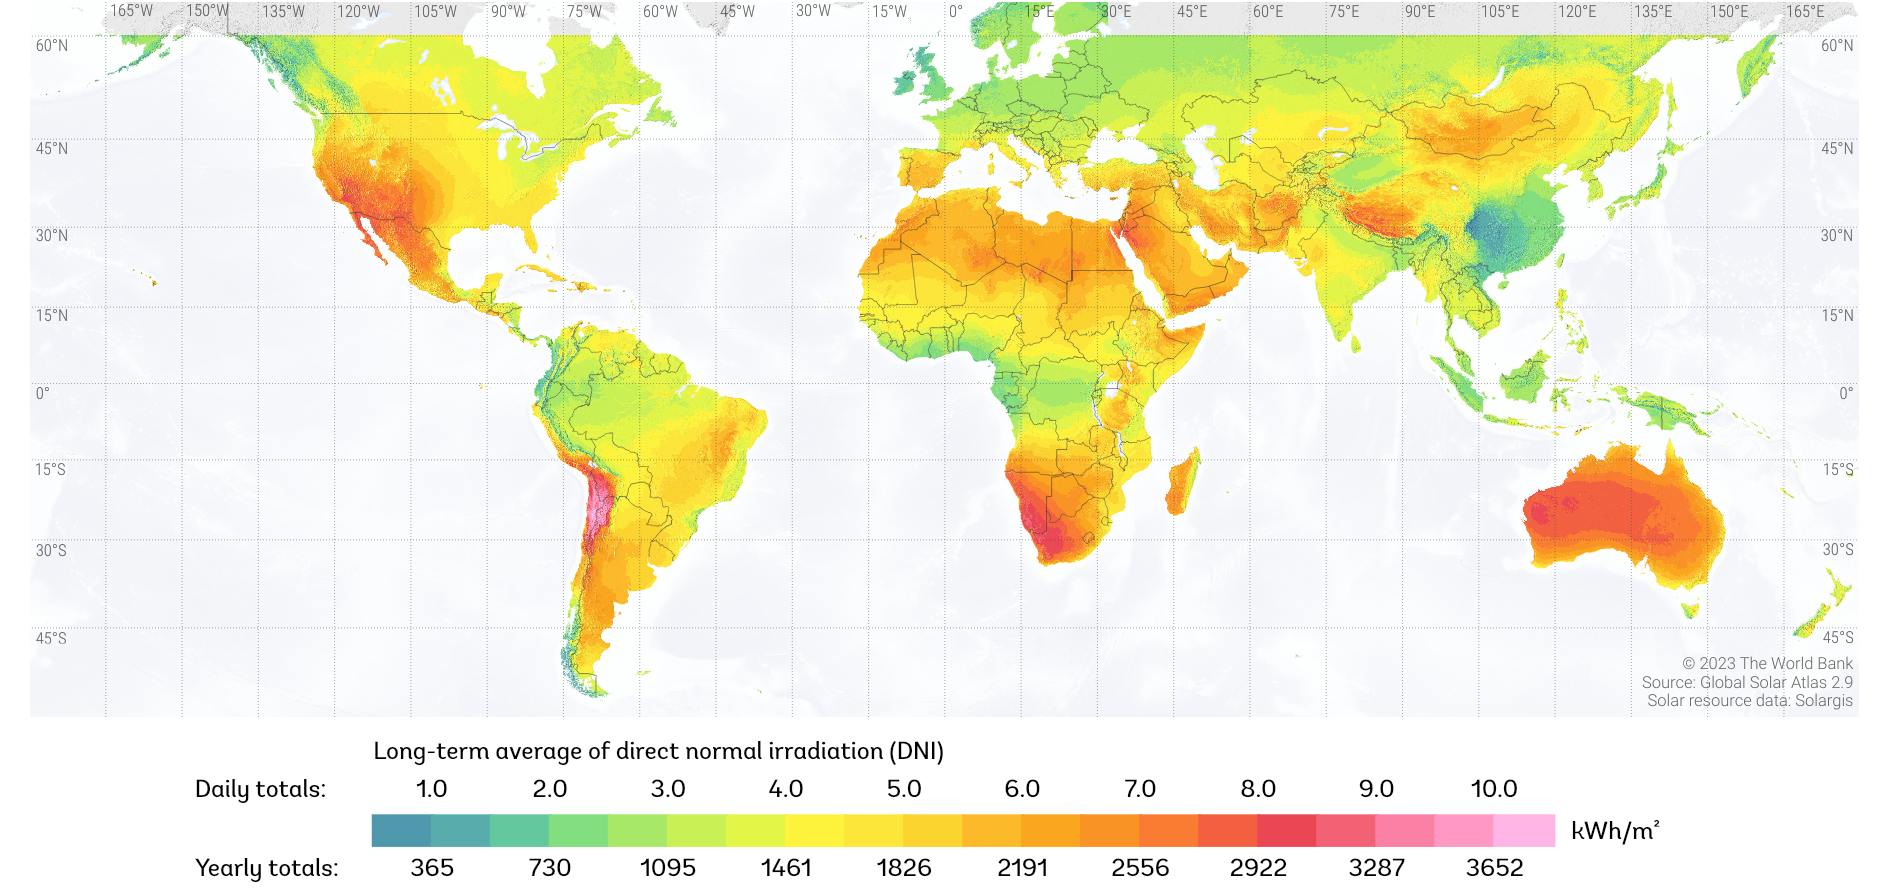
\includegraphics[width=1\textwidth]{img/diseno/dni.png}
    \caption{Mapa mundial del índice de radiación directa normal (\acrshort{dni}) mundial \cite{globalsolar}}
    \label{fig:dni}
\end{figure}

\vspace{3mm}

\begin{figure}[H]
    \centering
    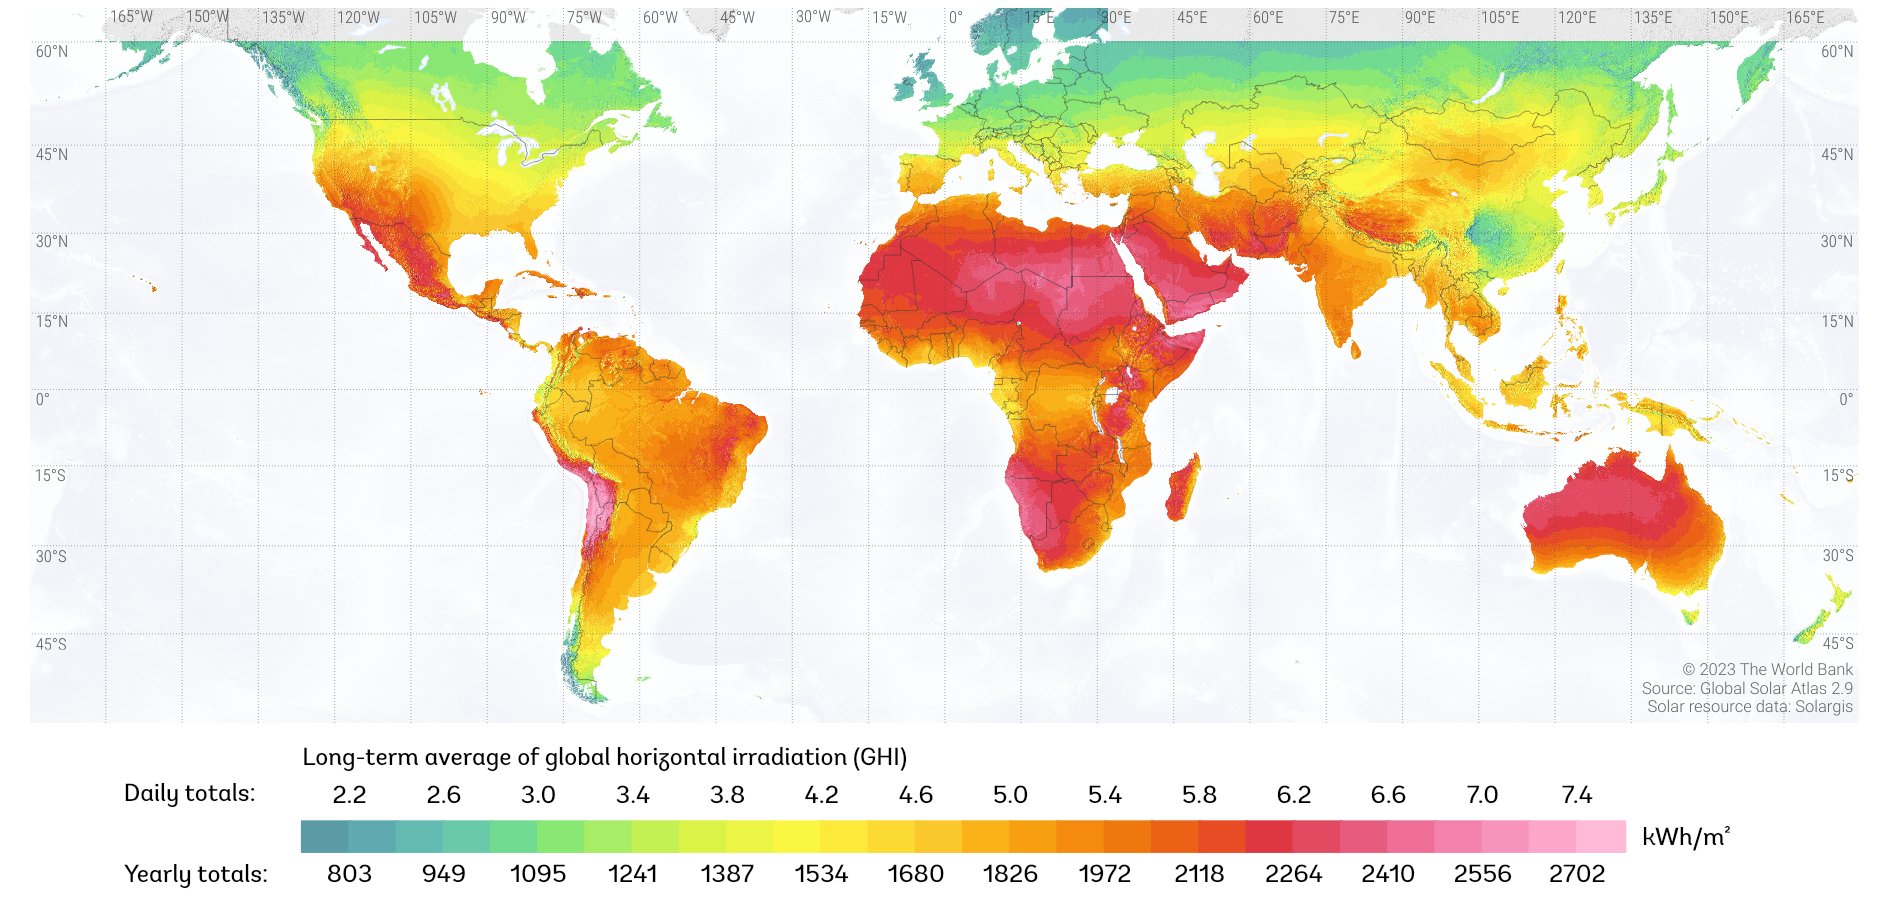
\includegraphics[width=1\textwidth]{img/diseno/ghi.png}
    \caption{Mapa del índice de radiación horizontal global (\acrshort{ghi}) mundial \cite{globalsolar}}
    \label{fig:ghi}
\end{figure}

\vspace{3mm}

\pagebreak

\begin{figure}[H]
    \centering
    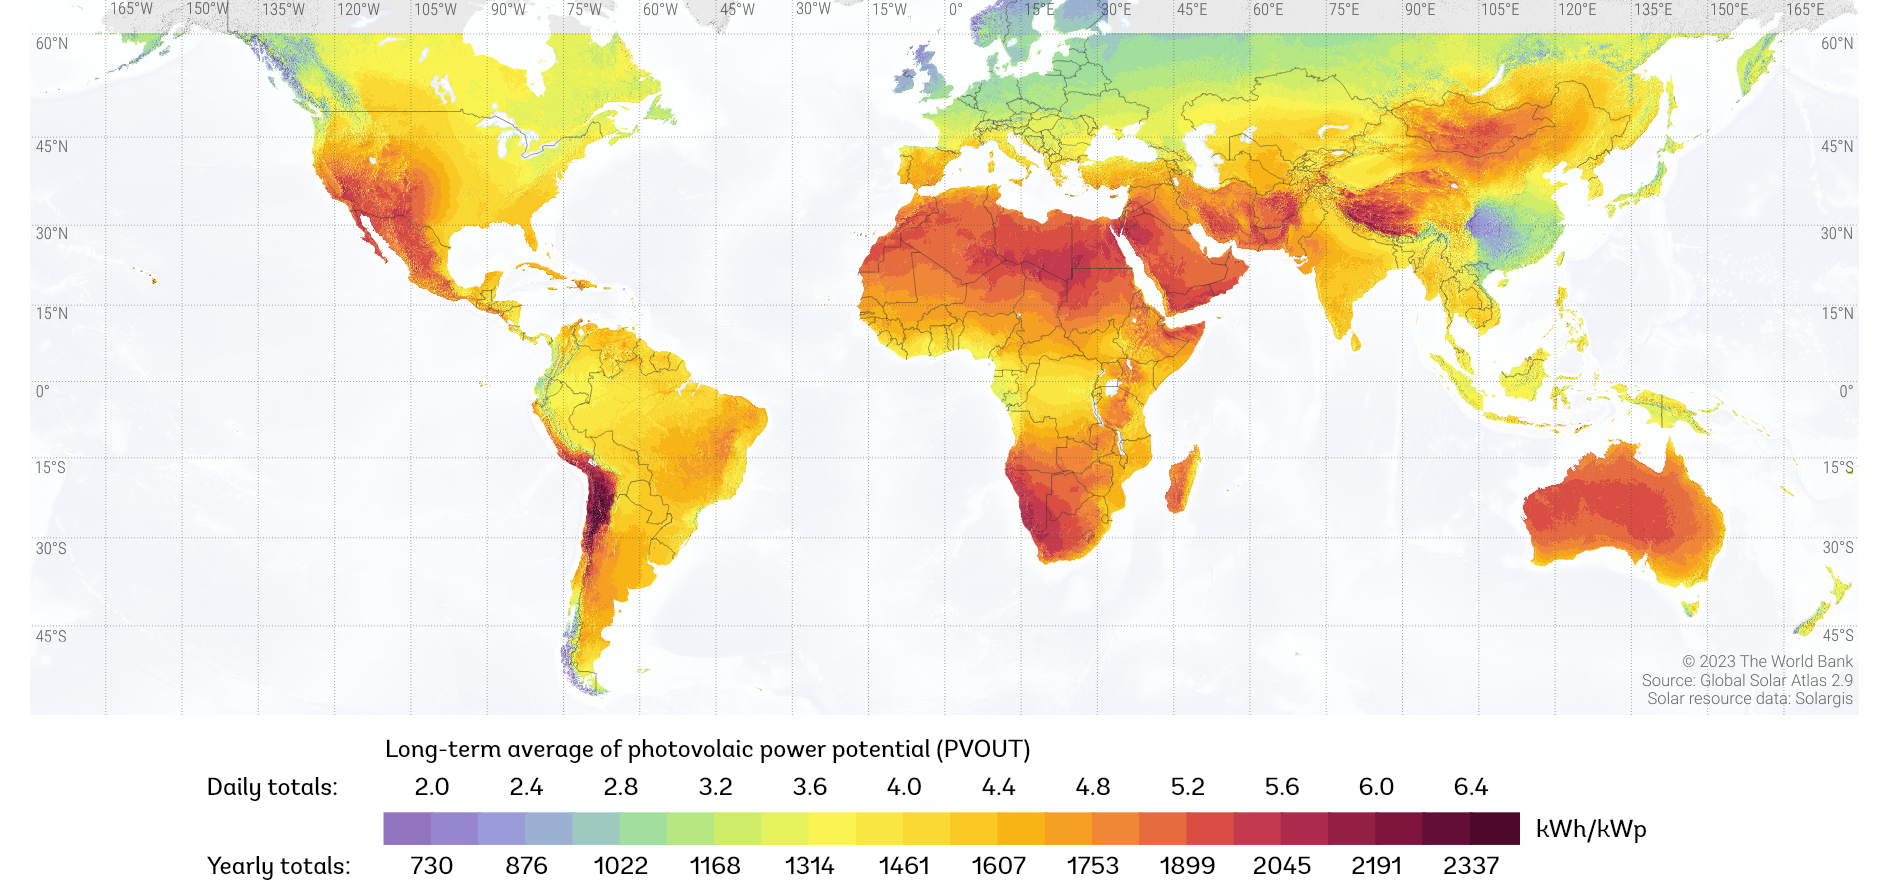
\includegraphics[width=1\textwidth]{img/diseno/photovoltaic.png}
    \caption{Mapa del potencial de producción energética fotovoltaica (\acrshort{pvout}) mundial \cite{globalsolar}}
    \label{fig:photo}
\end{figure}

\subsubsection{Análisis de resultados de radiación}

De la misma forma, lo anterior se hace patente para el caso de la isla de Madeira, como se puede visualizar en las Figuras \ref{fig:madeiradni}, \ref{fig:madeiraghi} y \ref{fig:madeirapvout}. Desde la plataforma \textit{Global Solar Atlas} también se extraen y se recogen en la Tabla \ref{tab:global} los valores de los índices de radiación, configurados específicamente para la localización de la ciudad de Funchal. 

\vspace{5mm}

\begin{table}[h!]
    \centering
    \begin{tabular}{|c|c|c|}
    \hline
    \rowcolor[HTML]{AAAAAA} 
    \multicolumn{1}{|c|}{\cellcolor[HTML]{AAAAAA}Parámetro} & \multicolumn{1}{c|}{\cellcolor[HTML]{AAAAAA}kWh/m²/día} & kWh/m²/año \\ \hline
    \gls{dni} & 3,698 & 1349,9 \\ \hline
    \gls{dif} & 2,038 & 743,8 \\ \hline
    \gls{ghi} & 4,345 & 1586,1 \\ \hline
    \gls{gti} & 4,730 & 1726,3 \\ \hline
    \end{tabular}
    \caption{Tabla de valores extraídos para cada índice de radiación en la ciudad de Funchal~\cite{globalsolar}}
    \label{tab:global}
\end{table}

\vspace{3mm}

Por tanto, se puede comprobar a través de estos valores y de la leyenda proporcionada en las figuras anteriores, que Funchal se percibe como una ciudad con un potencial de recursos solares medio alto. Esto es coherente con su localización subtropical y con la elevación del terreno. Es decir, al encontrarse en una zona de costa, ronda en valores cercanos a los 100 metros (concretamente 137 metros en la ubicación seleccionada) y se reduce ligeramente el nivel de energía solar captable respecto a otras zonas de la isla más montañosas.

\pagebreak

\begin{figure}[H]
    \centering
    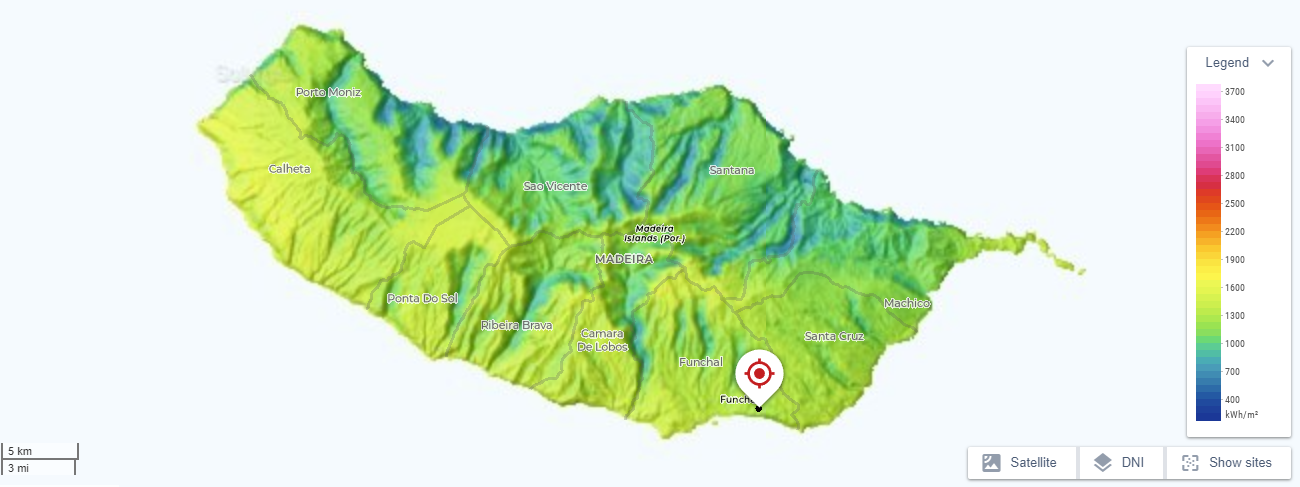
\includegraphics[width=1\textwidth]{img/diseno/madeiradni.png}
    \caption{Mapa del índice de radiación directa normal (\acrshort{dni}) de Madeira \cite{globalsolar}}
    \label{fig:madeiradni}
\end{figure}

\begin{figure}[H]
    \centering
    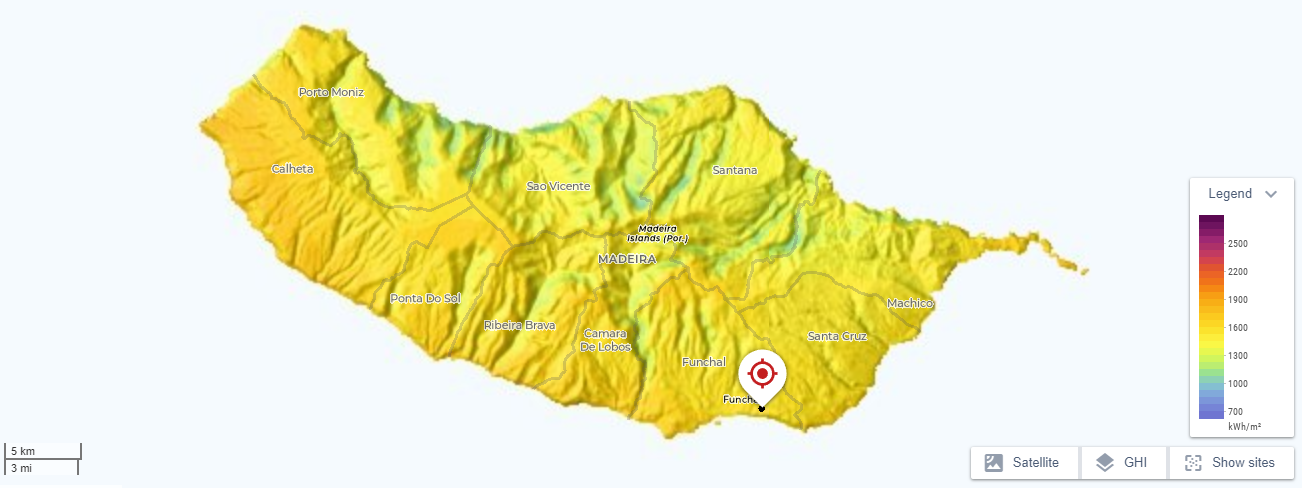
\includegraphics[width=1\textwidth]{img/diseno/madeiraghi.png}
    \caption{Mapa del índice de radiación horizontal global (\acrshort{ghi}) de Madeira \cite{globalsolar}}
    \label{fig:madeiraghi}
\end{figure}

\begin{figure}[H]
    \centering
    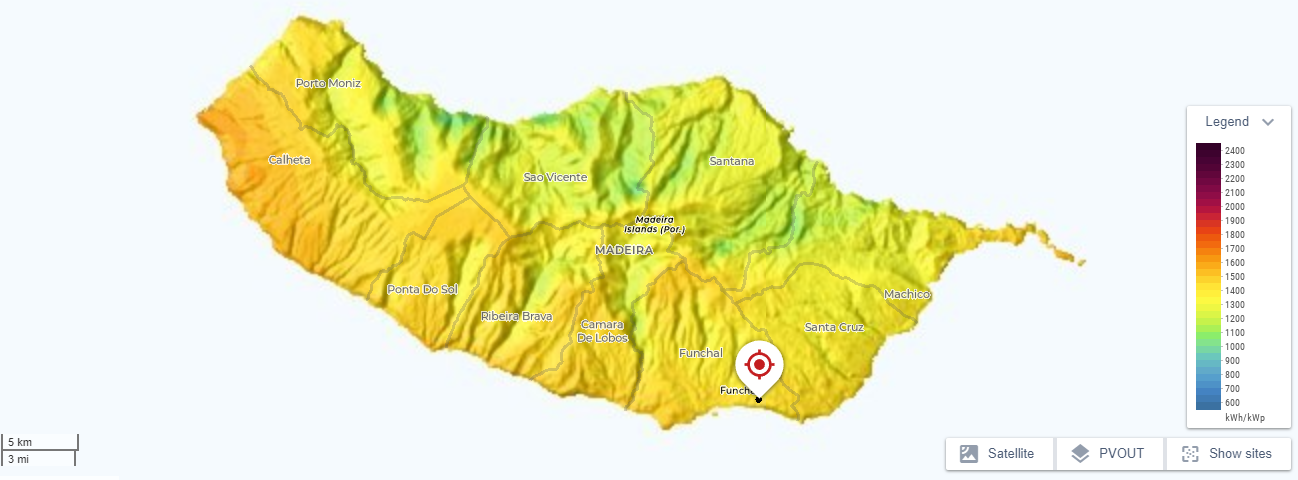
\includegraphics[width=1\textwidth]{img/diseno/madeirapvout.png}
    \caption{Mapa del potencial de producción energética fotovoltaica (\acrshort{pvout}) de Madeira \cite{globalsolar}}
    \label{fig:madeirapvout}
\end{figure}

\pagebreak

\subsubsection{Configuración y cuantificación del potencial energético de la ubicación}

Para calcular de forma aproximada la cantidad de energía que supondría la instalación de un sistema fotovoltaico en una vivienda ubicada en la ciudad de Funchal, es preciso configurar primero los siguientes parámetros a través de la plataforma:

\begin{itemize}
    \item Tipo y tamaño de sistema fotovoltaico: Se permite seleccionar entre un sistema enfocado a una vivienda, a un edificio comercial o a una planta solar de grandes dimensiones. En este caso, se toma como base el estudio de producción energética en un entorno residencial. Es preciso indicar que en la plataforma la configuración de un sistema fotovoltaico para un entorno residencial no considera la opción de almacenamiento de electricidad.
    \item Capacidad de instalación: Se toma una capacidad máxima de generación de 4kWp (kilovatios pico) para el sistema. En otros términos, este valor determina la cantidad de energía que producirían los paneles en condiciones óptimas.
    \item Azimut \cite{azimut}: Se determina como el ángulo de orientación horizontal y, en función de su valor, define la proyección de los paneles solares en dirección norte, sur, este u oeste. Se indica un valor de 180º para establecer una orientación hacia el sur. 
    \item Inclinación: La plataforma establece como ángulo óptimo para la localización de Funchal un ángulo de 26º, por lo que se configura la instalación de los paneles solares sobre rieles sujetos a un tejado con esta misma inclinación.
\end{itemize}

\subsubsection{Análisis de resultados de potencia}
\label{sec:analisisglobal}

Una vez configurados los parámetros expuestos, se obtienen como resultados la trayectoria solar diaria y los perfiles de radiación y generación fotovoltaica diarios y mensuales para la ubicación de Funchal. En la Figura \ref{fig:azimut} se representa la trayectoria solar diaria, en la que se puede visualizar la comparación de la elevación que percibe el sol en función del instante del año, siendo máxima durante el solsticio de junio, y mínima, durante el de diciembre. En el caso del equinoccio, se sigue una curva con valores promedios, al existir una igualdad entre las horas de día y las de noche. 

\vspace{3mm}

Por otro lado, en la Figura \ref{fig:average}, se modelan gráficamente los valores totales mensuales, tanto de producción energética, como de radiación directa normal \gls{dni} para visualizar la correlación existente entre los mismos en los distintos meses del año. El valor promedio máximo energético se alcanza en el mes de julio, con un valor de 565kWh, ocurriendo de la misma forma para el valor máximo de radiación, cuyo alcance es de 163,7kWh/m² para este mes.

\begin{figure}[H]
    \centering
    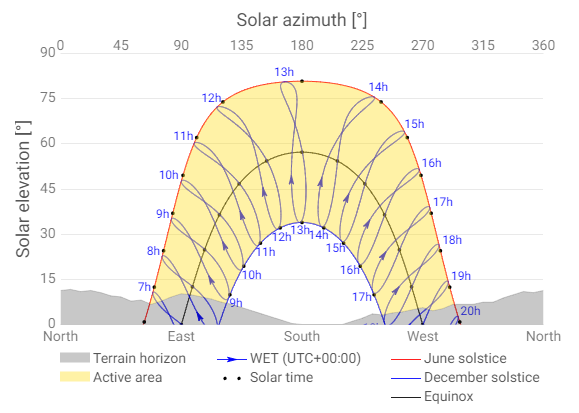
\includegraphics[width=0.9\textwidth]{img/diseno/azimut.png}
    \caption{Representación de la trayectoria solar percibida en la localización de la ciudad de Funchal \cite{globalsolar}}
    \label{fig:azimut}
\end{figure}

\vspace{3mm}

\begin{figure}[H]
    \centering    
    \begin{subfigure}{0.5\linewidth}
        \centering
        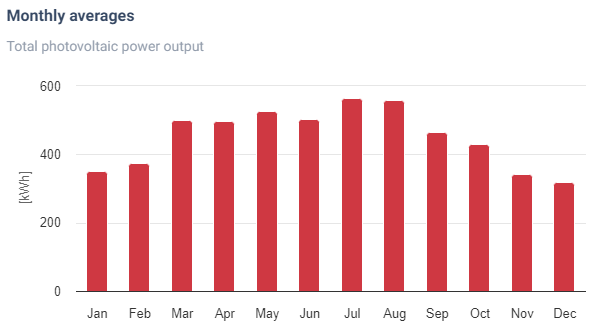
\includegraphics[width=\linewidth,height=5cm]{img/diseno/averagepvout.png}
        \label{fig:averagepvout}
    \end{subfigure}\hfill
    \begin{subfigure}{0.5\linewidth}
        \centering
        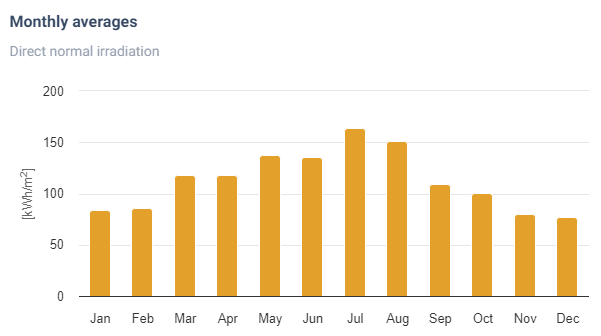
\includegraphics[width=\linewidth,height=5cm]{img/diseno/averagedni.png}
        \label{fig:averagedni}
    \end{subfigure}    
    \caption{Comparación de valores totales mensuales de producción energética fotovoltaica (\acrshort{pvout}) respecto a la radiación directa normal (\acrshort{dni}) \cite{globalsolar}}
    \label{fig:average}
\end{figure}

De la misma forma, se representan en la Figura \ref{fig:averagehour} los perfiles diarios propromedios de radiación y generación fotovoltaica en función del mes del año, en los cuales se encuentran valores máximos en las horas centrales de los meses de julio y agosto. 

\pagebreak

\begin{figure}[H]
    \centering    
    \begin{subfigure}{0.75\linewidth}
        \centering
        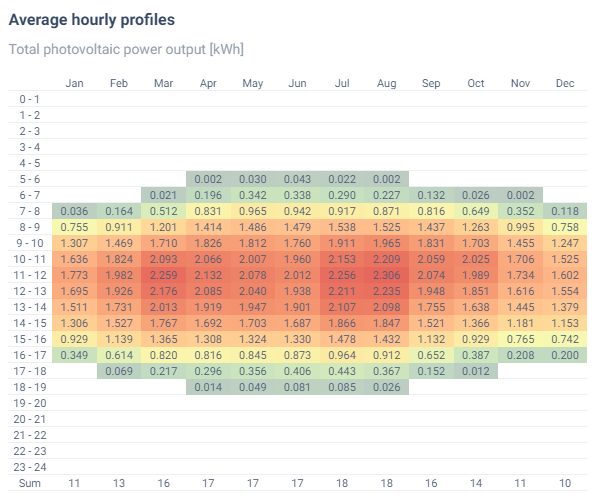
\includegraphics[width=\linewidth]{img/diseno/averagepvouthour.png}
        \label{fig:averagepvouthour}
    \end{subfigure}\hfill

    \begin{subfigure}{0.75\linewidth}
        \centering
        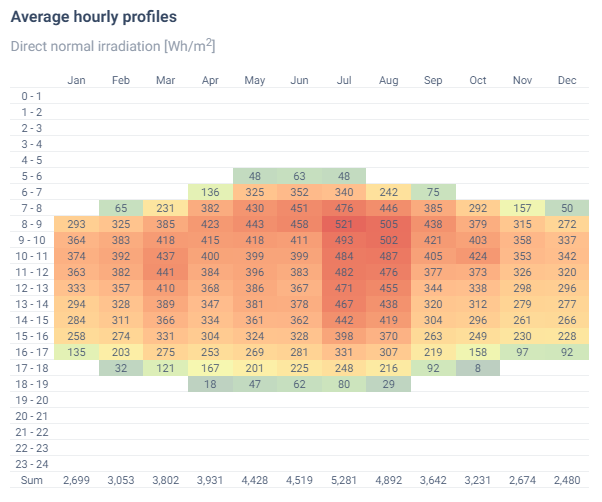
\includegraphics[width=\linewidth]{img/diseno/averagednihour.png}
        \label{fig:averagepdnihour}
    \end{subfigure}    
    \caption{Perfiles promedios de potencial de producción energética fotovoltaica (\acrshort{pvout}) y de radiación directa normal (\acrshort{dni}) \cite{globalsolar}}
    \label{fig:averagehour}
\end{figure}

\pagebreak

Por lo tanto, tomando en consideración los parámetros configurados y los resultados obtenidos, se puede cuantificar finalmente, que la instalación de un sistema fotovoltaico en un edificio residencial de Funchal proporcionaría en un año una generación de energía promedia igual a 5433kWh y un valor acumulado de \gls{dni} equivalente a 1719,4 kWh/m².

\vspace{3mm}

%ver pag 26-31 technical report -> losses


% Total photovoltaic power output and Global tilted irradiation (4)
% 0.015MWh per day 4.711kWh/m2 per day
% 5433kWh per year 1719.4 kWh/m2 per year

% \begin{figure}[H]
%     \centering
%     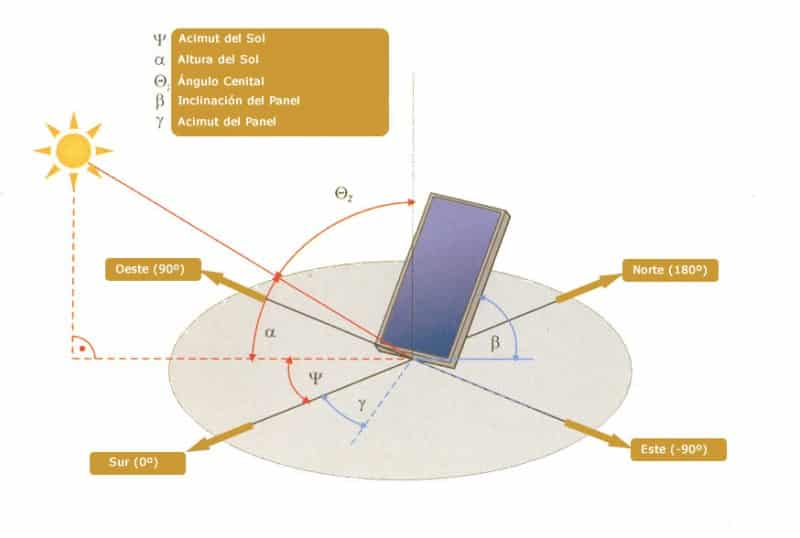
\includegraphics[width=0.8\textwidth]{img/diseno/orient.jpg}
%     \caption{Geometría solar para la instalación de paneles solares \cite{azimut}}
%     \label{fig:orient}
% \end{figure}

% •	Ver pdf PV Systems Performance in Madeira, gráficas interesantes, indica zonas de madeira con mayor producción
% •	Ver Solar Energy Resource in Madeira Islands, gráficas interesantes


\subsection{Creación del dataset de producción (\textit{PVWatts})}
\label{sec:pvw}

Una vez que se han concretado a modo de análisis las características geográficas, climáticas y energéticas de la localización seleccionada en la ciudad de Funchal, se procederá a realizar el paso dedicado a la obtención de los datos de producción fotovoltaica por medio de la simulación. Para ello, se hará uso de la herramienta online \textit{PVWatts}\footnote{https://pvwatts.nrel.gov/pvwatts.php} \cite{pvwatts}, proporcionada por el \gls{nrel}, que se trata del laboratorio nacional del Departamento de Energía de Estados Unidos. 

\vspace{3mm}

De la misma forma que se ha operado con la plataforma \textit{Global Solar Atlas} (ver Sección \ref{sec:global}), en el caso de \textit{PVWatts}, también se requiere indicar a la entrada las características relativas a la ubicación seleccionada y a la configuración del sistema de paneles fotovoltaicos que se desea. 

\vspace{3mm}

En cuanto a la primera, la herramienta \textit{PVWatts}, a diferencia de \textit{Global Solar Atlas}, provee un mapa mundial que se rige por celdas, en función de la localización de las bases de datos del \gls{nrel}. En el caso de este \gls{tfm}, se cuenta con la fortuna de que se dispone de una de estas bases en la misma ciudad de Funchal, concretamente en las coordenadas 32,65°N, 16,92°W. En este contexto, es preciso comentar que esta característica se tuvo en cuenta para definir la localización exacta de instalación del sistema fotovoltaico en la plataforma \textit{Global Solar Atlas} (ver Sección \ref{sec:global}). Por lo tanto, no se requieren ajustes adicionales en estos términos.  

\subsubsection{Configuración de los parámetros de entrada}

Con el objetivo de conseguir a la salida de la simulación unos datos que sean coherentes y acordes al análisis realizado anteriormente en la Sección \ref{sec:analisisglobal}, es imprescindible replicar y ajustar de la forma más precisa posible los valores de los parámetros de entrada de la herramienta: 

\pagebreak

\begin{itemize}
    \item Tamaño del sistema fotovoltaico y capacidad de instalación: Por defecto, \textit{PVWatts} determina una capacidad de 4kWp, por lo que coincide directamente con la definida en \textit{Global Solar Atlas}. Además, se especifica la relación existente entre este valor y el tamaño del sistema de la siguiente manera:
    \[\frac{4 \, \text{kW}}{1 \, \text{kW/m}^2 \times 0,16} = 25 \, \text{m}^2\]
    Donde se representa que, para obtener una eficiencia del 16\% del sistema (eficiencia por defecto), se requiere un área de 25 m² para los módulos solares. Es decir, este valor no representa el área total del sistema fotovoltaico, ya que para ello habría que añadir el cálculo del espacio que se necesita establecer entre cada uno de los paneles DC o el tamaño de los inversores AC que se instalarían.
    \item Índice de cobertura del suelo: Se define como la relación entre el área de superficie del módulo y el área del suelo (tejado en el caso de una vivienda) ocupado en total. El valor predeterminado es de 0,4, lo que supone que, teniendo un área efectiva de 25 m², se necesitará un área total de 62,5 m².
    \item Ratio DC/AC: Haciendo referencia al tamaño de los inversores AC, es preciso exponer que estos limitan la salida de la energía del conjunto para que haya un correcto funcionamiento. La herramienta cuantifica por defecto para la localización, una relación 1,2 entre el tamaño de array de paneles y los inversores de corriente alterna. Por lo tanto, en este caso, estos contarían con una capacidad teórica de 3,33kW. Si se pretendiera realizar una instalación a gran escala se necesitarían ratios de hasta 1,5.
    \item Azimut: De la misma forma que en la configuración en la plataforma \textit{Global Solar Atlas}, se define un azimut de 180º, orientando los paneles hacia el sur.
    \item Inclinación: \textit{Global Solar Atlas}, en el caso de localizar el sistema fotovoltaico en la ciudad de Funchal, establecía como ángulo óptimo de inclinación un valor de 26º.
    \item Tipo de módulos: Se selecciona el tipo estándar, basado en silicio cristalino y con una cobertura de vidrio con revestimiento antireflectante. Aproximadamente, cuenta con una eficiencia nominal del 19\%.
    \item Tipo de array: Se especifica de forma simplificada un tipo de array fijo, que no siga el movimiento del sol mediante ejes de rotación, sino que mantenga sus valores de inclinación y de azimut configurados. En la Figura \ref{fig:array}, se describe el funcionamiento de cada tipo de array.
\end{itemize}


\begin{figure}[H]
    \centering
    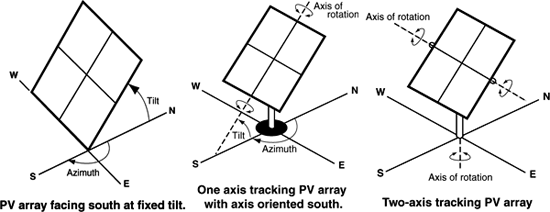
\includegraphics[width=0.9\textwidth]{img/diseno/array.png}
    \caption{Representación de las diferentes opciones de array que permite configurar la herramienta \textit{PVWatts} \cite{pvwatts}}
    \label{fig:array}
\end{figure}

\subsubsection{Configuración de las pérdidas del sistema real}

Una de las ventajas de uso que permite la herramienta \textit{PVWatts} es la posibilidad de estimar las pérdidas totales que tendría el sistema en la realidad. Esto es importante para que los resultados de la simulación que se va a realizar sean lo más parecidos a los que se obtendrían mediante la medición del sistema real. Para ello, se deben configurar cada una de las pérdidas parciales de la siguiente manera:

\begin{itemize}
    \item Suciedad: Debido a la escasez de precipitaciones y a la presencia de calima que se experimenta en la isla, se determina un valor de un 2\%.
    \item Sombreado: Se reduce la radiación solar que incide en los paneles si se producen sombras por objetos cercanos o por la propia de los módulos si se colocan en fila. Es decir, estos crean sombras sobre los de la fila adyacente. El cálculo se realiza a partir de la gráfica expuesta en la Figura \ref{fig:sombra}. Por lo tanto, como se ha definido un tipo de array fijo con una inclinación de 26º y un valor de índice de cobertura del suelo de 0,4, se determina aproximadamente un valor de pérdidas por sombra igual a un 3\%.
    \item Nieve: Teniendo en cuenta las características climáticas de la ciudad de Funchal, debido a su localización en una zona subtropical, se determinan pérdidas del 0\%.
    \item Discordancia: Son pérdidas eléctricas debido a las diferencias que se producen por imperfecciones en la fabricación de los módulos. Esto tiene como consecuencia que cada uno de ellos presente características I-V que varíen ligeramente entre sí. La herramienta proporciona un valor predeterminado del 2\%.
    \pagebreak
    \item Cableado y conexiones: Pérdidas resistivas en el cableado y en las conexiones entre módulos, inversores y otros elementos del sistema con un valor por defecto del 2\% y del 0,5\%, respectivamente.
    \item Degradación inducida por la luz: Se trata del efecto de reducción de potencia que se produce durante los primeros meses de funcionamiento del sistema fotovoltaico. El valor predeterminado es 1,5\%.
    \item Precisión del fabricante: Son pérdidas, generalmente bajas, que vienen definidas por la precisión del fabricante en el proceso de estudio de eficiencia de los paneles. Se determina un 1\%.
    \item Disponibilidad: Se añaden las pérdidas que se producen a partir de los mantenimientos que se requieren a lo largo del tiempo y que causan paradas en el funcionamiento del sistema. Se provee un valor por defecto del 3\%.
\end{itemize}

Finalmente, las pérdidas totales del sistema se pueden cuantificar a partir de la siguiente expresión:
    \[\textit{Losses} = (1-0,02) \times (1-0,03) \times (1-0,02) \times (1-0,02) 
    \times (1-0,005) \times (1-0,015) \times (1-0,01) \times (1-0,03)\]
    \[100\% \times (1-\textit{Losses}) = 14,08\%\]

\begin{figure}[H]
    \centering
    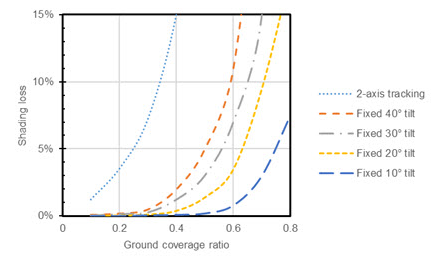
\includegraphics[width=0.85\textwidth]{img/diseno/sombra.png}
    \caption{Gráfica para el cálculo de las pérdidas por sombreado en la herramienta \textit{PVWatts}~\cite{pvwatts}}
    \label{fig:sombra}
\end{figure}

\subsubsection{Análisis de resultados de la simulación}
\label{sec:resultadossimu}

Una vez se ha concluido con la configuración necesaria, se procede a ejecutar la simulación en la herramienta y a adquirir a la salida los resultados de la misma. Se obtienen dos datasets que replican un año completo de mediciones: uno con los valores totales mensuales (ver Tabla \ref{tab:pvwattsdataset2}) y otro, con un conjunto de muestras que proporcionan información de cada hora (ver Tabla \ref{tab:pvwattsdataset}). 

\vspace{3mm}

Como se puede visualizar, en ambas tablas se proporcionan los valores de potencia DC y AC, que corresponden a la salida del módulo solar (\textit{DC Array Output}) y de los inversores (\textit{AC System Output}), respectivamente. En el caso de la Tabla (ver Tabla \ref{tab:pvwattsdataset}), se incluye de forma adicional toda la información climática y ambiental de cada instante.

\vspace{3mm}

\begin{table}[h!]
    \centering
    \begin{tabular}{|c|c|c|}
    \hline
    \rowcolor[HTML]{AAAAAA} 
    \multicolumn{1}{|c|}{\cellcolor[HTML]{AAAAAA}Campo} & \multicolumn{1}{c|}{\cellcolor[HTML]{AAAAAA}Descripción} & Unidades \\ \hline
    \textit{Month} & Mes de la muestra & - \\ \hline
    \textit{Daily POA Irradiance} & Índice de radiación en el plano del array & kWh/m2/day \\ \hline 
    \textit{DC Array Output} & Potencia de salida DC del array & kWh \\ \hline
    \textit{AC System Output} & Potencia de salida AC del sistema & kWh \\ \hline
    \end{tabular}
    \caption{Dataset con valores totales mensuales \cite{pvwatts}}
    \label{tab:pvwattsdataset2}
\end{table}

\vspace{1mm}

\begin{table}[h!]
    \centering
    \begin{tabular}{|c|c|c|}
    \hline
    \rowcolor[HTML]{AAAAAA} 
    \multicolumn{1}{|c|}{\cellcolor[HTML]{AAAAAA}Campo} & \multicolumn{1}{c|}{\cellcolor[HTML]{AAAAAA}Descripción} & Unidades \\ \hline
    \textit{Month} & Mes de la muestra & - \\ \hline
    \textit{Day} & Día de la muestra & - \\ \hline
    \textit{Hour} & Hora de la muestra & - \\ \hline
    %\textit{Beam Irradiance} & Índice de radiación directa normal (\gls{dni}) & W/m2 \\ \hline 
    \textit{Diffuse Irradiance} & Índice de radiación difusa (\gls{dif}) & W/m2 \\ \hline
    \textit{Plane of Array Irradiance} & Índice de radiación en el plano del array (\acrshort{poa}) & W/m2 \\ \hline 
    \textit{Ambient Temperature} & Temperatura ambiente & C \\ \hline
    \textit{Wind Speed} & Velocidad del viento & m/s \\ \hline
    \textit{Albedo} & Índice de reflectividad de la superficie & - \\ \hline
    \textit{Cell Temperature} & Temperatura de las células solares & C \\ \hline
    \textit{DC Array Output} & Potencia de salida DC del array & W \\ \hline
    \textit{AC System Output} & Potencia de salida AC del sistema & W \\ \hline
    \end{tabular}
    \caption{Dataset con muestras adquiridas por hora \cite{pvwatts}}
    \label{tab:pvwattsdataset}
\end{table}

\vspace{3mm}

Teniendo en cuenta las tablas anteriores, en este paso será imprescindible comprobar que los datos finales obtenidos presentan coherencia respecto al estudio previo y que encajan además, con el análisis de los resultados de la plataforma \textit{Global Solar Atlas}, realizado en la Sección \ref{sec:analisisglobal}. 

\vspace{3mm}

Por ello, en primera instancia, se va a proceder a poner el foco en los valores de radiación directa normal \gls{dni}. La herramienta \textit{PVWatts}, como se puede ver en la Tabla \ref{tab:pvwattsdataset2}, no proporciona directamente información mensual sobre este parámetro, sino sobre el índice de radiación en el plano del array (del inglés \gls{poa}), que se calcula a partir de la expresión \cite{poa}:

\begin{equation}
    \gls{poa} = \gls{dni} \cdot \cos(\theta) 
\end{equation}

    Donde:
\begin{itemize}
    \renewcommand{\labelitemi}{}
    \item \( \theta \) es el ángulo de inclinación configurado, que en este caso sería de 26º.
\end{itemize}

\vspace{3mm}

Por lo tanto, se pueden calcular los valores de \gls{dni} a partir de los de \gls{poa} dados por el dataset. Mediante la librería \textit{matplotlib} de \textit{Python}, se representa la Figura \ref{fig:averagereal} para visualizar los valores totales mensuales, tanto de producción energética, como de radiación directa normal \gls{dni}. El valor máximo energético se alcanza en el mes de julio, con un valor de 517,8kWh, ocurriendo de la misma forma para el valor promedio máximo de radiación, cuyo alcance es de 181,1kWh/m² para este mes. Por tanto, volviendo a la Sección \ref{sec:analisisglobal} y, específicamente a la \ref{fig:average}, se puede determinar que los valores obtenidos en la simulación son muy precisos respecto al estudio previo.

\vspace{3mm}

\begin{figure}[H]
    \centering    
    \begin{subfigure}{0.5\linewidth}
        \centering
        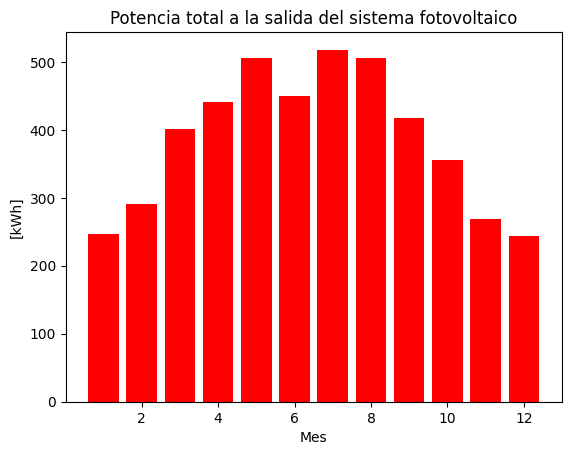
\includegraphics[width=\linewidth,height=6.5cm]{img/diseno/averagepvoutreal.png}
        \label{fig:averagepvoutreal}
    \end{subfigure}\hfill
    \begin{subfigure}{0.5\linewidth}
        \centering
        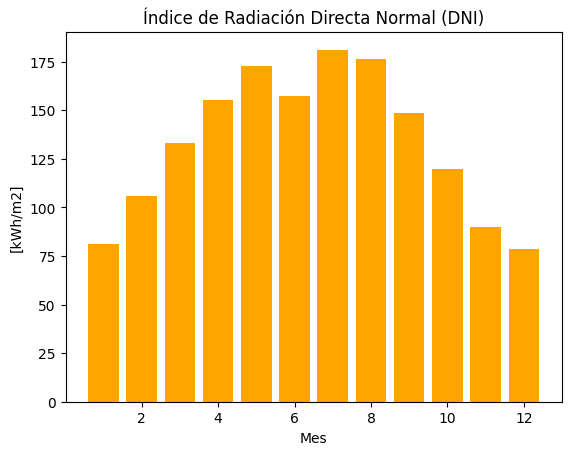
\includegraphics[width=\linewidth,height=6.5cm]{img/diseno/averagednireal.png}
        \label{fig:averagednireal}
    \end{subfigure}    
    \caption{Comparación de valores totales mensuales de producción energética fotovoltaica (\acrshort{pvout}) respecto a la radiación directa normal (\acrshort{dni}) a partir de los resultados de la simulación}
    \label{fig:averagereal}
\end{figure}

\pagebreak

Aparte de las gráficas realizadas, se expone la Tabla \ref{tab:globalvspvwatts} para llevar a cabo de una forma correcta la comparación entre los valores estudiados en \textit{Global Solar Atlas} y los resultantes de la simulación en \textit{PVWatts}. Como se puede ver, existe un menor error entre los valores respectivos a la radiación que entre los valores de potencia producida. Las diferencias percibidas provienen principalmente por las pérdidas configuradas, ya que al final los resultados de la simulación son mucho más cercanos al caso real que los percibidos teóricamente. 

\begin{sidewaystable}
    \centering 
    \begin{tabularx}{\textheight}{|c|XX|XX|}
        \hline
        \rowcolor[HTML]{EFEFEF} 
        \cellcolor[HTML]{C0C0C0} & \multicolumn{2}{c|}{\cellcolor[HTML]{C0C0C0}Producción energética fotovoltaica (PVOUT) [kWh]} & \multicolumn{2}{c|}{\cellcolor[HTML]{C0C0C0}Índice de Radiación Directa Normal (DNI) [kWhm2]} \\ \cline{2-5} 
        \rowcolor[HTML]{C0C0C0} 
        \multirow{-2}{*}{\cellcolor[HTML]{C0C0C0}Mes} & \multicolumn{1}{c|}{\cellcolor[HTML]{C0C0C0}Global Solar Atlas} & PVWatts & \multicolumn{1}{c|}{\cellcolor[HTML]{C0C0C0}Global Solar Atlas} & PVWatts \\ \hline
        \textit{Enero} & \multicolumn{1}{c|}{350,2} & \multicolumn{1}{c|}{247,1} & \multicolumn{1}{c|}{83,7} & \multicolumn{1}{c|}{81,1} \\ \hline
        \textit{Febrero} & \multicolumn{1}{c|}{374,0} & \multicolumn{1}{c|}{291,4} & \multicolumn{1}{c|}{85,5} & \multicolumn{1}{c|}{105,7} \\ \hline
        \textit{Marzo} & \multicolumn{1}{c|}{500,8} & \multicolumn{1}{c|}{401,9} & \multicolumn{1}{c|}{117,9} & \multicolumn{1}{c|}{132,8} \\ \hline
        \textit{Abril} & \multicolumn{1}{c|}{497,9} & \multicolumn{1}{c|}{441,3} & \multicolumn{1}{c|}{117,9} & \multicolumn{1}{c|}{155,0} \\ \hline
        \textit{Mayo} & \multicolumn{1}{c|}{526,5} & \multicolumn{1}{c|}{505,9} & \multicolumn{1}{c|}{137,3} & \multicolumn{1}{c|}{172,7} \\ \hline
        \textit{Junio} & \multicolumn{1}{c|}{502,5} & \multicolumn{1}{c|}{449,6} & \multicolumn{1}{c|}{135,6} & \multicolumn{1}{c|}{157,4} \\ \hline
        \textit{Julio} & \multicolumn{1}{c|}{565,5} & \multicolumn{1}{c|}{517,8} & \multicolumn{1}{c|}{163,7} & \multicolumn{1}{c|}{181,1} \\ \hline
        \textit{Agosto} & \multicolumn{1}{c|}{558,6} & \multicolumn{1}{c|}{505,5} & \multicolumn{1}{c|}{151,6} & \multicolumn{1}{c|}{176,1} \\ \hline
        \textit{Septiembre} & \multicolumn{1}{c|}{465,3} & \multicolumn{1}{c|}{417,4} & \multicolumn{1}{c|}{109,3} & \multicolumn{1}{c|}{148,7} \\ \hline
        \textit{Octubre} & \multicolumn{1}{c|}{429,0} & \multicolumn{1}{c|}{356,3} & \multicolumn{1}{c|}{100,2} & \multicolumn{1}{c|}{119,5} \\ \hline
        \textit{Noviembre} & \multicolumn{1}{c|}{343,7} & \multicolumn{1}{c|}{268,8} & \multicolumn{1}{c|}{80,2} & \multicolumn{1}{c|}{90,1} \\ \hline
        \textit{Diciembre} & \multicolumn{1}{c|}{318,6} & \multicolumn{1}{c|}{243,4} & \multicolumn{1}{c|}{76,9} & \multicolumn{1}{c|}{78,6} \\ \hline
    \end{tabularx}
    \caption{Tabla de comparación de los valores totales mensuales de producción energética fotovoltaica (\acrshort{pvout}) y de radiación directa normal (\acrshort{dni}) de las dos herramientas (valores teóricos y simulados)}
    \label{tab:globalvspvwatts}
\end{sidewaystable}


\vspace{3mm}

Por lo tanto, a través del sumatorio de todos los valores mensuales de producción energética, se puede cuantificar finalmente, que un sistema fotovoltaico real localizado en la ciudad de Funchal, proveería aproximadamente un total de 4417kWh al año. Este valor representa un 81,3\% del obtenido teóricamente (5433kWh) en la Sección \ref{sec:analisisglobal} y viene justificado en gran parte por las pérdidas introducidas. Por otro lado, en el caso del \gls{dni}, con la herramienta \textit{PVWatts} se obtiene un total anual equivalente a 1598,8 kWh/m², suponiendo un 92,9\% del valor teórico (1719,4 kWh/m²).

\vspace{3mm}

Es preciso tener en cuenta las diferencias que presentan las herramientas \textit{Global Solar Atlas} y \textit{PVWatts} en sus algoritmos de cálculo, ya que cada una de ellas asignará pesos diferentes a los parámetros de entrada, incidiendo parcialmente en los resultados. No obstante, a partir de los valores anteriores y de la Tabla \ref{tab:globalvspvwatts}, se puede determinar de forma concluyente que la simulación realizada es coherente con el estudio previo, cumpliendo así el objetivo principal de esta Sección.

\clearpage